\documentclass[11pt]{beamer}                                                                                               \usetheme{Boadilla}
\usepackage{graphicx}
\usepackage{subfigure}
\usepackage[english]{babel}
\usepackage{times}
\usepackage[T1]{fontenc}
\usepackage{ctex}

\usefonttheme[onlymath]{serif}


\begin{document}
	%\begin{frame}
	\title[PT Summary]{5.18PT汇报}
	\author[Tang Yi]{} % 显示作者
	\institute[]{} % 设置学院机构
	\date{\today}  % 显示日期
	\begin{frame}
		\titlepage
	\end{frame}
	\section{T6 Non-contact Resistance}
	
	\begin{frame}
		\sectionpage
		The responses of an LRC circuit driven by an AC source can be changed by inserting either a non-magnetic metal rod or a ferromagnetic rod into the inductor coil. How can we obtain the magnetic and electric properties of the inserted rod from the circuit's responses?
	\end{frame}
	\subsection{Theory}
	\begin{frame}[fragile]
		\frametitle{初步理论}
		\,\,\,\,\,\,\,\,\,\,\,\,\,通过往线圈里面插入介质棒，改变线圈的电感和电阻，其中改变量和介质的电磁学特性有关。我们通过测量线圈在介质棒插入前后的电感和电阻来确定介质的特性。
		
		\,\,\,\,\,\,\,\,\,\,\,\,\,插入介质棒后，介质中会有几种效应共同作用。下面是具体推导，推导中暂时忽略边界效应。
		
	\end{frame}
	
	\begin{frame}[fragile]
		\frametitle{场方程分析}
		由Maxwell方程，线圈中的交流电产生的交变磁场会在介质棒中产生涡流，产生能量损耗，对整个系统而言即为电阻变大。
		
		\centerline{$\nabla \times \vec{E}=\dfrac{1}{\sigma}\nabla \times \vec{j}=-\dfrac{\partial \vec{B}}{\partial t}$}
		
		\centerline{$\vec{B_0}=\mu_0 n I \vec{e_B}$}
		
		\centerline{$\vec{B}=\vec{B_0}+\vec{B'}$}
		
		即我们还需要求出感应电流产生的磁场$\vec{B'}$。
		\centerline{$\nabla \times \vec{H'}=\vec{j}+\dfrac{\partial \vec{D}}{\partial t}$}
		
		代入上式，有
		\centerline{$\nabla \times (\nabla \times \vec{H'})=\nabla(\nabla \cdot \vec{H'})-\nabla^2 \vec{H'}=-\dfrac{1}{\mu} \nabla^2 \vec{B'}=-\dfrac{1}{\mu} \nabla^2 \vec{B}$}
		
		代入化简后，有
		\centerline{$\nabla^2 \vec{B}+\epsilon \mu \dfrac{\partial^2 \vec{B}}{\partial t^2}=-\mu \sigma \dfrac{\partial \vec{B}}{\partial t}$}
		
		显然，这是有外界驱动的电磁波方程。当然，在非高频的情况下，可以认为其不向外辐射电磁波，即忽略$\vec{B'}$对导体中$\vec{j}$的影响。
		
	\end{frame}
	

	\begin{frame}[fragile]
		\frametitle{近似场方程分析}
		由于已经忽略$\vec{B'}$对导体中$\vec{j}$的影响，我们可通过
		
		\centerline{$\nabla \times \vec{j}=-\sigma \dfrac{\partial \vec{B_0}}{\partial t}$}
		
		直接解得$\vec{j}$，求解过程如下
		
	
		代入后两侧对到轴线$r$的面上积分，得到
		
		\centerline{$\dfrac{1}{\sigma} \displaystyle\int_{ S}\nabla \times \vec{j} \cdot \mathrm{d}\vec{S}=-\displaystyle\int_{ S} \dfrac{\partial \vec{B_0}}{\partial t}\cdot \mathrm{d}\vec{S}=-\mu_0 n\displaystyle\int_{ S} \dfrac{\partial I}{\partial t} \vec{e_B} \cdot \mathrm{d}\vec{S}$}
		
		等式左边用Stoke公式换为环积分，再直接积分出来，有
		
		\centerline{$\dfrac{1}{\sigma} \displaystyle\oint_{\partial S} \vec{j} \cdot \mathrm{d}\vec{l}=\dfrac{2 \pi r j}{\sigma}=\mu_0 n \pi r^2 \dfrac{\mathrm{d}I}{\mathrm{d} t}$}
		
		整理得
		\centerline{$j=\dfrac{1}{2} \mu_0 n r \dfrac{\mathrm{d}I}{\mathrm{d} t}$} 
	\end{frame}
	
	\begin{frame}[fragile]
		\frametitle{近似场方程分析}
			我们假设距轴线$r$的电流密度是$j(r)$，介质半径$r_s$，由则可得到
		
		\centerline{$\vec{B'}(r)=-\displaystyle \int_{r}^{r_s} \mu j(r) \mathrm{d} r \vec{e_B}=-\dfrac{\mu_0 \mu n}{4} \dfrac{\mathrm{d}I}{\mathrm{d} t}(r_s^2-r^2)\vec{e_B}$}
		
		而涡流所产生的电动势等效到线圈上就是一个额外的电压降，这个额外的电压我们可以用Faraday电磁感应定律很快得到。
		\centerline{$\mathcal{E}=-\dfrac{\mathrm{d}\varPsi}{\mathrm{d} t}=-nl\dfrac{\mathrm{d}\varPhi}{\mathrm{d} t}=-nl\dfrac{\mathrm{d}}{\mathrm{d} t}\displaystyle \int_{0}^{r_s}2 \pi r B'(r)\mathrm{d} r=-\dfrac{1}{8}\pi \mu_0 \mu \sigma n^2 l r_s^4\dfrac{\mathrm{d}^2I}{\mathrm{d} t^2}$}
		
		当我们输入任意交变电流，实际上都能通过Founier变化看作是无穷多个正弦波的叠加。
		
		对正弦波$I=I_0 \sin(\omega t +\phi)$，代入后发现和额外的电压成正比，这个比例系数为:
		\centerline{$R_p=\dfrac{1}{8}\pi \mu_0 \mu \sigma n^2 l r_s^4 \omega^2$}
		
		由于实际线圈的电压是本身线圈的电阻产生的电压和感抗产生的电压和插入介质棒后涡流产生的电压线性叠加造成的。那么这个量纲等同电阻的比例系数即使在这一频率下插入介质棒后多得到的$\Delta R$。
	\end{frame}
	
	\begin{frame}[fragile]
		\frametitle{近似场方程分析}
		除了线圈的电阻改变，其等效电感也发生了变化。电感的计算相对简单，直接考虑介质带来的修正效应即可。
		
		对之前的线圈，电感
		\centerline{$L=\mu_0 n^2 S l$}
		
		插入介质后，电感
		\centerline{$L'=\mu_0 n^2 (S-S_p) l+\mu n^2 S_p l$}
		
		则得到
		\centerline{$L_p=\mu_0 (\mu_r-1) n^2 S_p l$}
	\end{frame}
	
	\begin{frame}[fragile]
		\frametitle{具体金属杆分析}
		对于铝杆这样的杆来说，$\mu_r \approx 1$，得到
		
		\centerline{$R_p=\dfrac{1}{8}\pi \mu_0^2 \sigma n^2 l r_s^4 \omega^2$}
		\centerline{$L_p=0$}
		
		对于铁氧体杆这样的杆来说，$\sigma \approx 0$得到
		\centerline{$R_p=0$}
		\centerline{$L_p=\mu_0 (\mu_r-1) n^2 S_p l$}
		
		对于铁杆这样的杆来说，得到
		\centerline{$R_p=\dfrac{1}{8}\pi \mu_0 \mu \sigma n^2 l r_s^4 \omega^2$}
		\centerline{$L_p=\mu_0 (\mu_r-1) n^2 S_p l$}	
	\end{frame}
	
	\subsection{Experience}
	\begin{frame}[fragile]
		\frametitle{具体数据的测定}
		\begin{figure}[h]%%图
			\centering  %插入的图片居中表示
			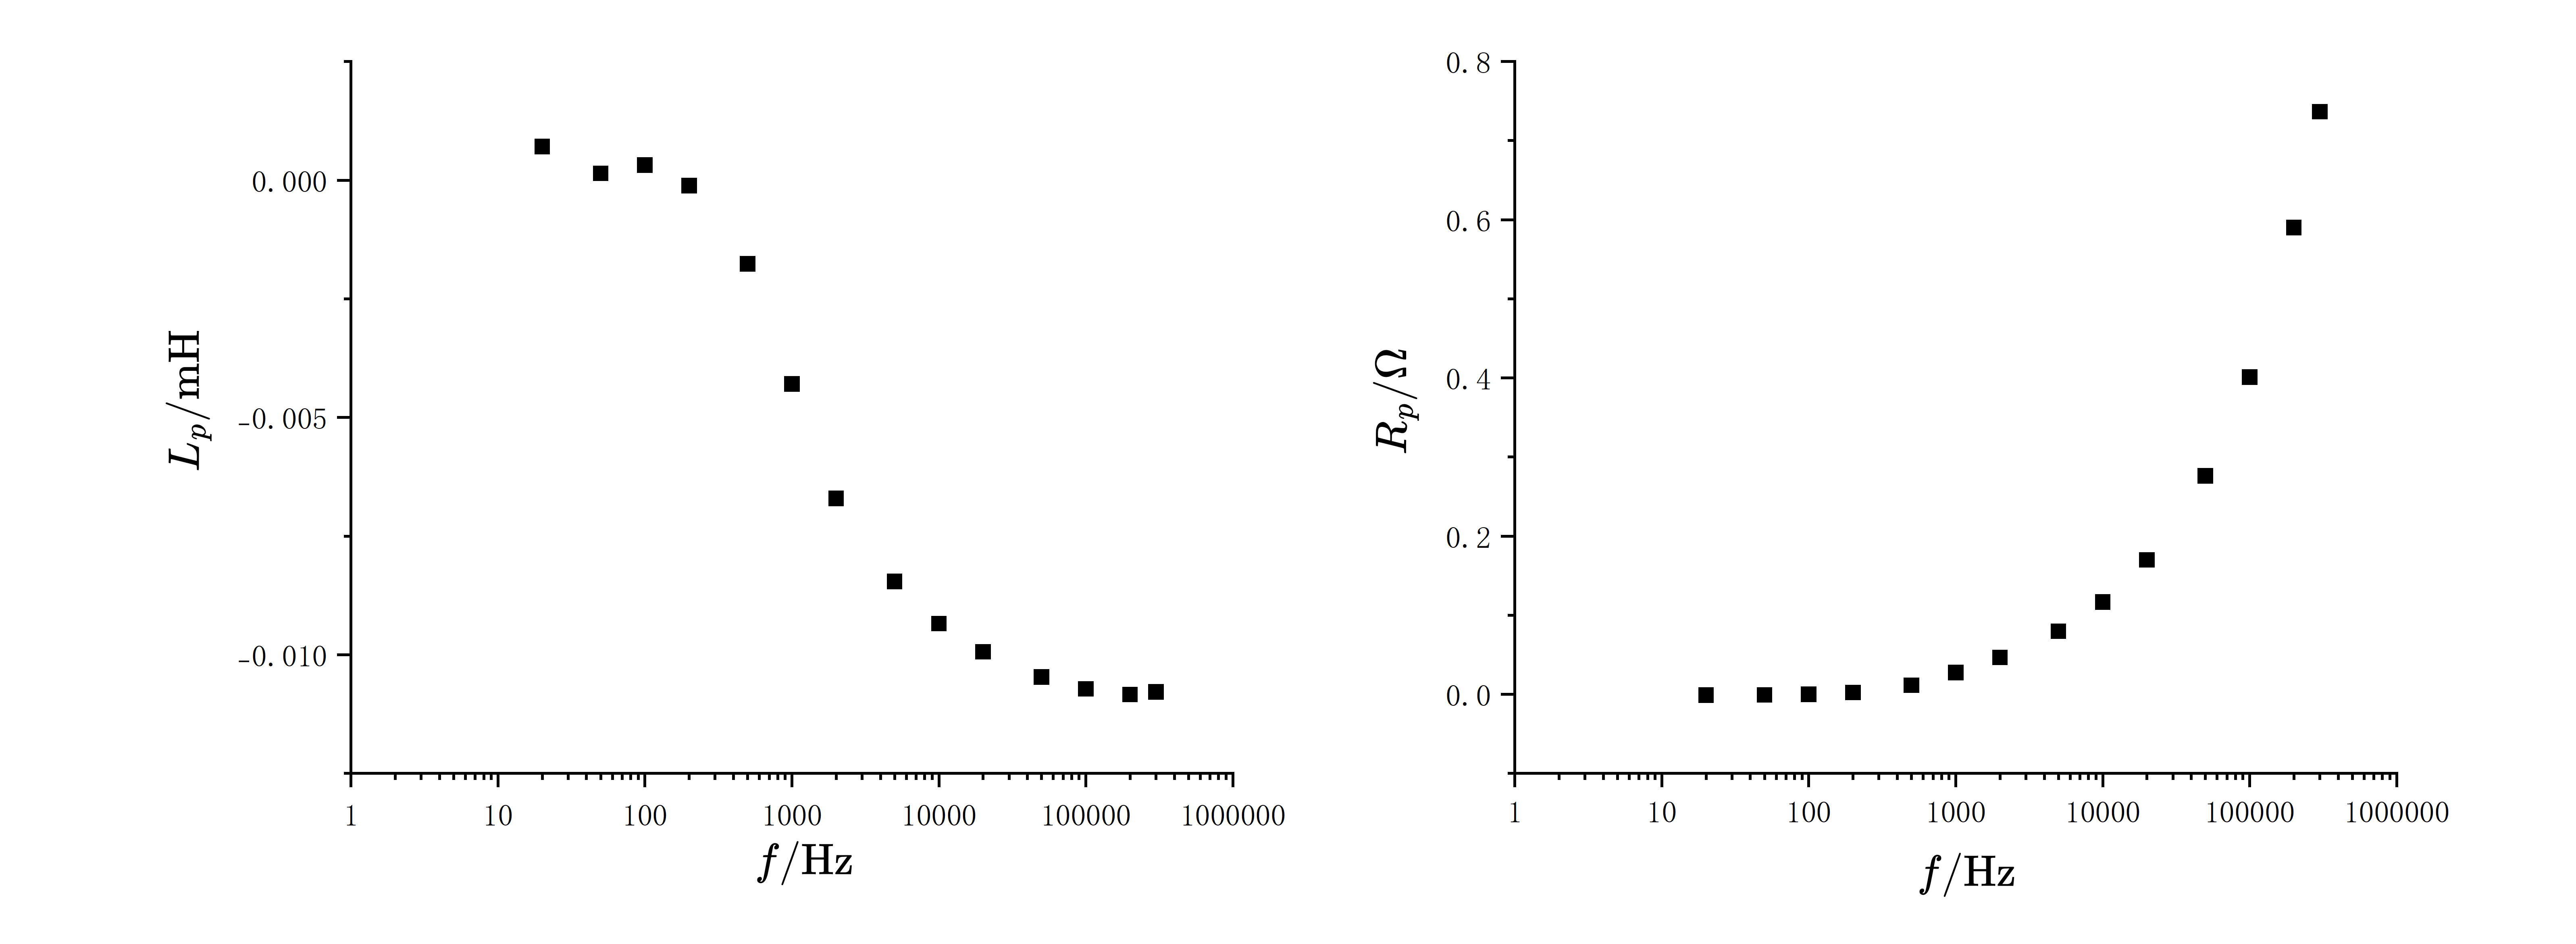
\includegraphics[width=1\linewidth]{5.18_J1.png}  
			\caption{Al棒在1V-AC下}  %图片的名称
		\end{figure}
	\end{frame}
	
	\begin{frame}[fragile]
		\frametitle{具体数据的测定}
		\begin{figure}[h]%%图
			\centering  %插入的图片居中表示
			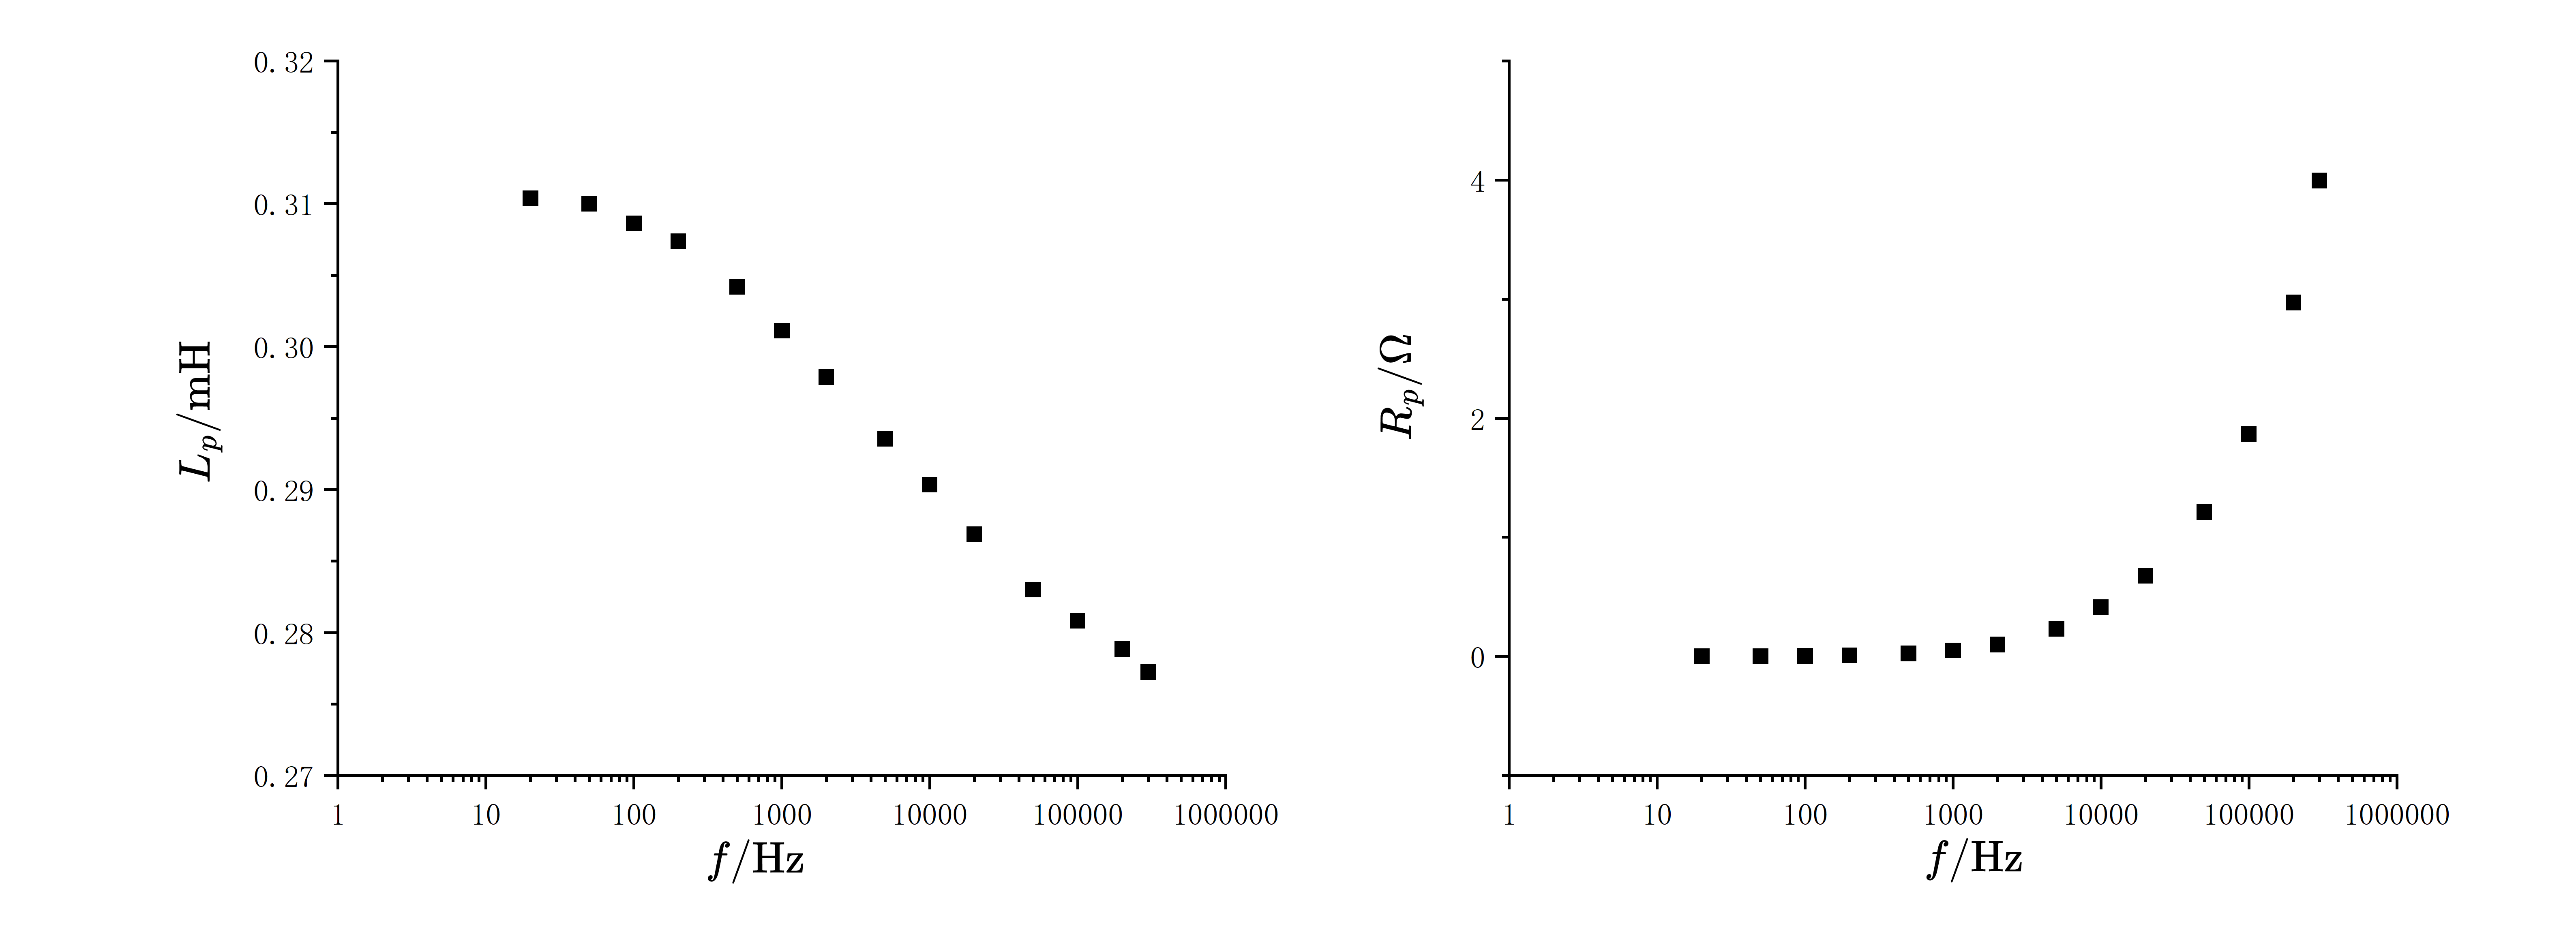
\includegraphics[width=1\linewidth]{5.18_J2.png}  
			\caption{Fe-O棒在1V-AC下}  %图片的名称
		\end{figure}
	\end{frame}
	
	\begin{frame}[fragile]
		\frametitle{具体数据的测定}
		\begin{figure}[h]%%图
			\centering  %插入的图片居中表示
			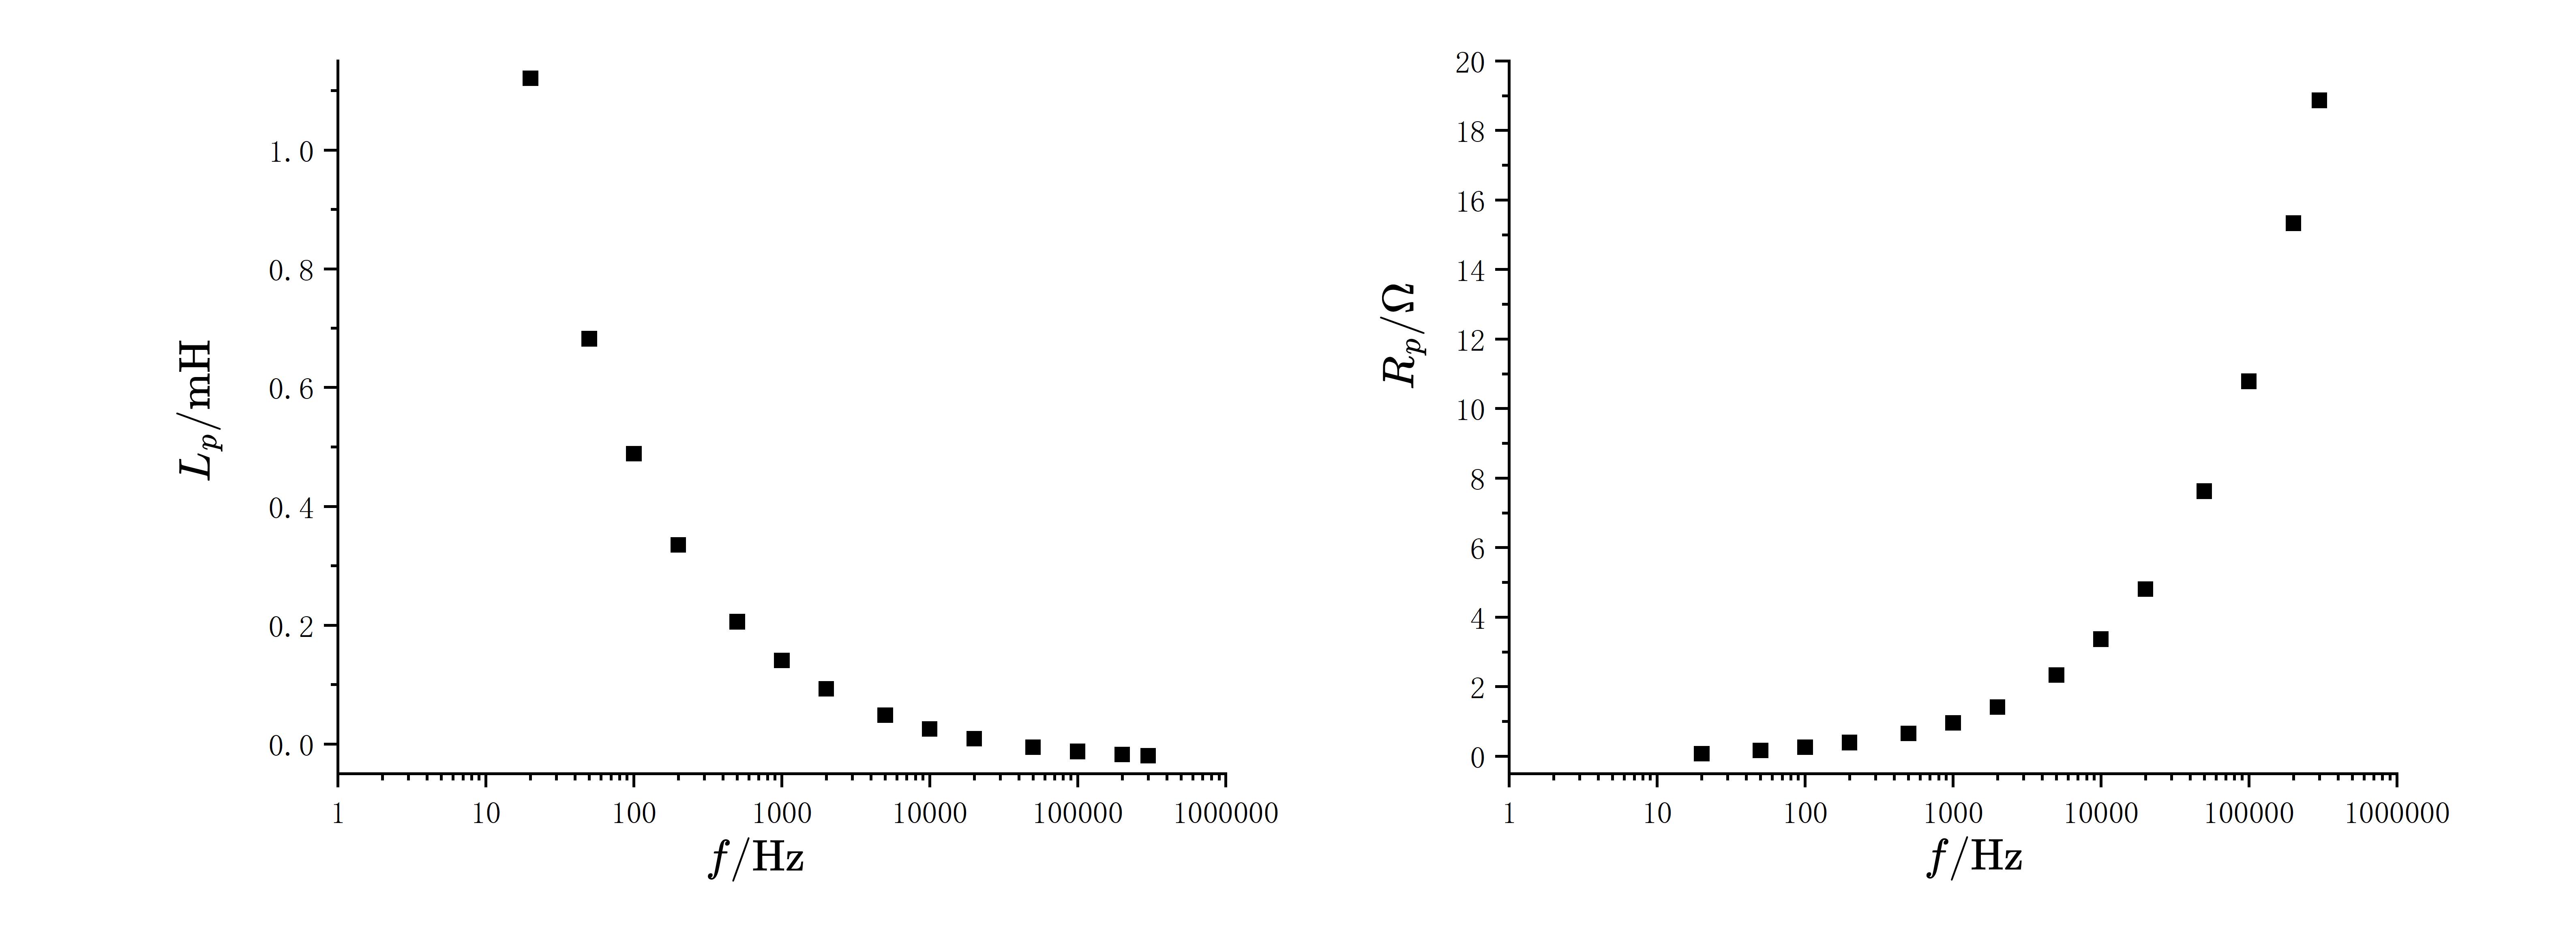
\includegraphics[width=1\linewidth]{5.18_J3.png}  
			\caption{Fe棒在1V-AC下}  %图片的名称
		\end{figure}
	\end{frame}
	
	\begin{frame}[fragile]
		\frametitle{需要后续思考的点}
		铝棒的$L_p<0$？
		
		铁棒的$L_p$有正有负？考虑磁滞？
		
		$R_p$曲线二次方拟合效果如何？边界效应影响有多大？
	\end{frame}

	\section{T14 Ruler Trick}

	\begin{frame}
		\sectionpage
		Place a ruler on the edge of a table, and throw a ball at its free end. The ruler will fall. However, if you cover a part of the ruler with a piece of paper and repeat the throw, then the ruler will remain on the table while the ball will bounce off it. Explain this phenomenon, and investigate the relevant parameters.
	\end{frame}
	
	\begin{frame}[fragile]
		\frametitle{理论修改}
		1.准静态修改为非静态过程。如何计算非静态过程模型中汽缸（纸面下）的压强？考虑流体力学。（后续查阅流体力学相关书籍）
		
		2.初速度模型修改为时变外力模型
		
		\centerline{$v=v_0 \rightarrow F=F_0 H(\tau -t)$}
		
		其中$H(t)$是阶跃函数。
		3.下一步准备给出模型和实际的各个参量的对应关系。
	\end{frame}
	
	\begin{frame}[fragile]
		\frametitle{尝试COMSOL建模计算}
		目前还没有完全做完，可以先看看半成品。
		\begin{figure}[h]%%图
			\centering  %插入的图片居中表示
			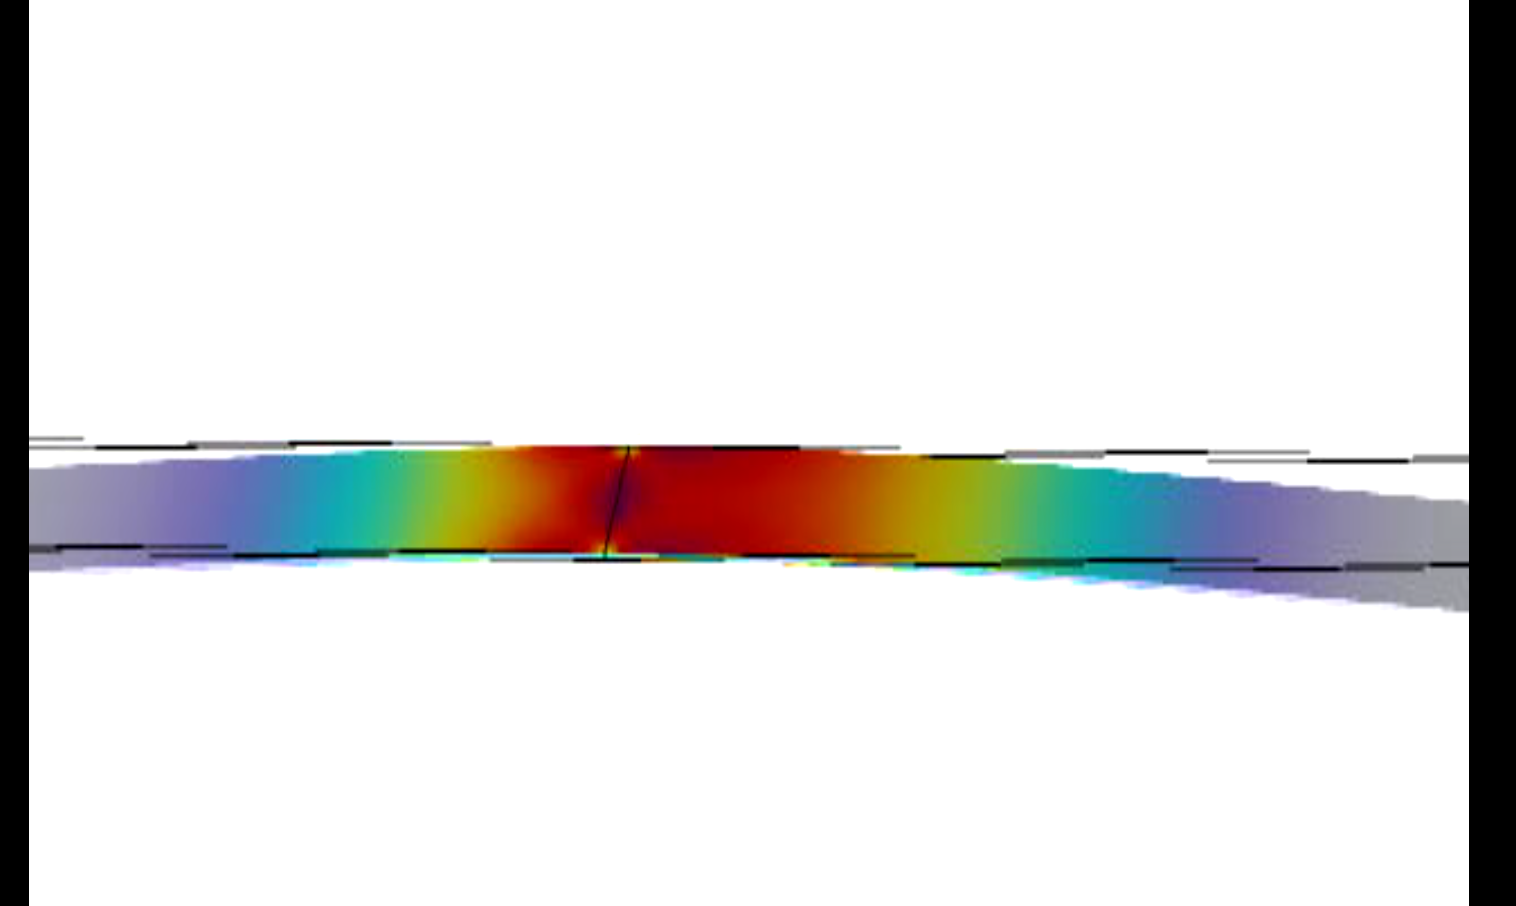
\includegraphics[width=1\linewidth]{5.18_J4.png}  
			%\caption{Fe-O棒在1V-AC下}  %图片的名称
		\end{figure}
	\end{frame}
	
	\begin{frame}[fragile]
		\frametitle{尝试COMSOL建模计算}
		\begin{figure}[h]%%图
			\centering  %插入的图片居中表示
			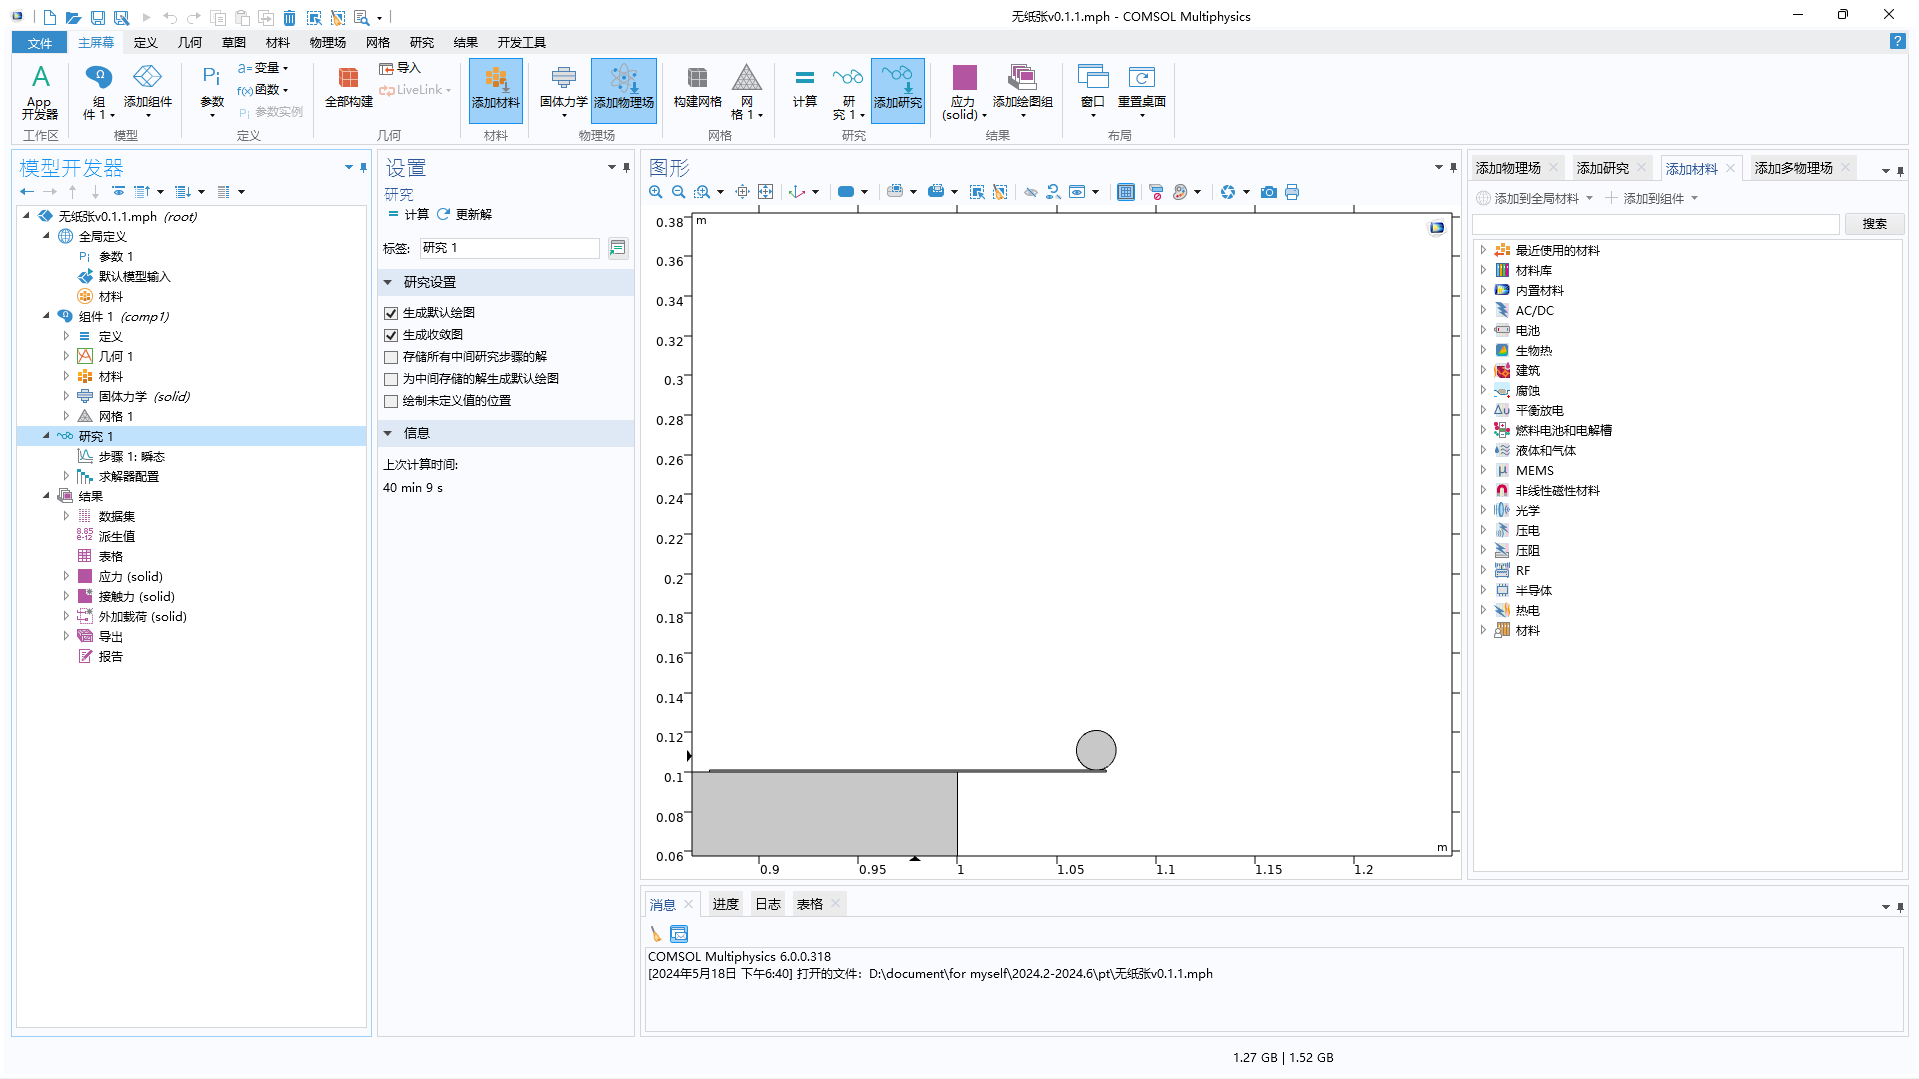
\includegraphics[width=1\linewidth]{5.18_J5.png}  
			%\caption{Fe-O棒在1V-AC下}  %图片的名称
		\end{figure}
	\end{frame}
	
	\begin{frame}[fragile]
		\frametitle{尝试COMSOL建模计算}
		尝试分别通过两种方式建模。
		
		一种是完全三维的复刻建模并加上流固耦合，另一种是通过建二维侧面图加约束条件来实现类似的效果。
	\end{frame}
	
	\begin{frame}[fragile]
		\frametitle{后续实验如何进展}
		实验测量严格化，让手测量造成的误差减小。
		
		可以通过改变架子，实验室有激光切割机可以切下相应的有机玻璃板，搭出来更准确的架子。（工程图还没来得及画）
		
		放尺子的架子可以设计个卡扣，科技楼一楼或物理楼三楼有3D打印机，可以先用Solidworks建模后在放在上面打印，保证每次位置的准确性。
		
		怎么改变气压？真空室能否搭出来表示存疑？
		
	\end{frame}
\end{document}